% Drawing 146/03-1 -- folder 146, batch 03, archive page 45 (PDF page 46).
% Transcription: un hexagone inscrit dans un cercle, de sommets marqués $\tilde{R}_1$, $\tilde{R}'_0$, $\tilde{R}_5$, $\tilde{R}'_4$, $\tilde{R}_3$, $\tilde{R}_2$ (ce dernier surchargé d'un $4$), le centre pointé ; les diagonales et quelques cordes sont tracées en tirets au crayon.
% Kind: circle with inscribed hexagon. Method 2 (schematic redraw from the facsimile). Status: ok.
% Notes: Hexagon inscribed in a pencil circle, centre pointed. The dashed chords are a reading of scattered pencil dashes: the six drawn here (R1-R3, R'0-R'4, R1-R5, R'0-R3, R2-R'4, R3-R5) are those whose dashes line up; others may be intended. The R~2 label is overwritten by a 4 (kept as R~2, as in the transcription).
% Coordinates: 1 unit = 1 mm = 1/100 of the crop width (bbox in page fractions: [0.11, 0.075, 0.42, 0.29]).
% Redrawn by Claude (claude-opus-5-5), issue #73 pilot, 2026-11-07; not checked by a human; not compiled (no TeX in the session).
% Rights: reproduces part of the work -- behind RENDER_TRANSCRIPTS, never published by itself.
\documentclass[tikz,border=3pt]{standalone}
\usepackage{amsmath,amssymb}
\usetikzlibrary{patterns,arrows.meta}
\tikzset{pencil/.style={black!45}, struck/.style={black!35}, mark/.style={circle,draw,inner sep=1.3pt}, pt/.style={circle,fill,inner sep=0.9pt}, opt/.style={circle,draw,fill=white,inner sep=1.1pt}}
\begin{document}
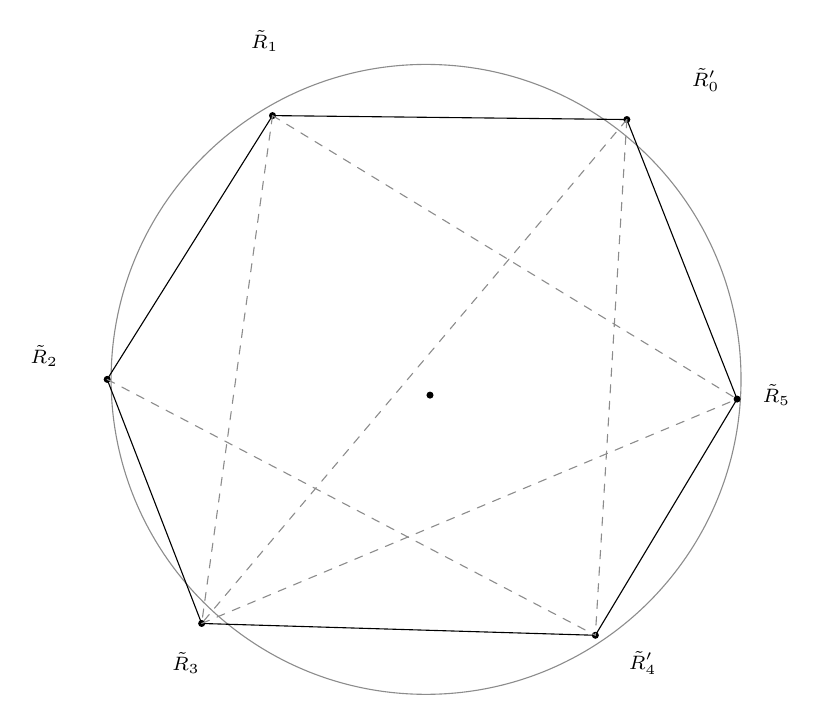
\begin{tikzpicture}[x=1mm,y=1mm,line cap=round,line join=round,font=\scriptsize]
\draw[pencil] (52.5,-55) circle[radius=40];
\draw (33,-21.5) -- (78,-22) -- (92,-57.5) -- (74,-87.5) -- (24,-86) -- (12,-55) -- cycle;
\node[pt] at (33,-21.5) {};
\node[pt] at (78,-22) {};
\node[pt] at (92,-57.5) {};
\node[pt] at (74,-87.5) {};
\node[pt] at (24,-86) {};
\node[pt] at (12,-55) {};
\node[pt] at (53,-57) {};
\draw[dashed,pencil] (33,-21.5) -- (24,-86);
\draw[dashed,pencil] (78,-22) -- (74,-87.5);
\draw[dashed,pencil] (33,-21.5) -- (92,-57.5);
\draw[dashed,pencil] (78,-22) -- (24,-86);
\draw[dashed,pencil] (12,-55) -- (74,-87.5);
\draw[dashed,pencil] (24,-86) -- (92,-57.5);
\node[inner sep=1pt] at (32,-12) {\scriptsize $\tilde{R}_1$};
\node[inner sep=1pt] at (88,-17) {\scriptsize $\tilde{R}'_0$};
\node[inner sep=1pt] at (97,-57) {\scriptsize $\tilde{R}_5$};
\node[inner sep=1pt] at (80,-91) {\scriptsize $\tilde{R}'_4$};
\node[inner sep=1pt] at (22,-91) {\scriptsize $\tilde{R}_3$};
\node[inner sep=1pt] at (4,-52) {\scriptsize $\tilde{R}_2$};
\end{tikzpicture}
\end{document}
